\documentclass[t,aspectratio=169]{beamer}

\usepackage{soul}
\usepackage{tikz}
\usepackage{multicol}
%\usepackage{gensymb}
\usepackage[utf8]{inputenc}

\usetikzlibrary{arrows.meta,decorations.markings,decorations.pathreplacing}


\usepackage{hyperref}
\hypersetup{
    colorlinks=true,
    linkcolor=blue,
    filecolor=magenta,      
    urlcolor=cyan,
    pdftitle={(KTXFI1EBNF) Physics I. Practice},
}

% ----------------------------------------------------------------------------------------------------------------------------------------

\title{\includegraphics[width=45pt]{oepecsetlogo.png}\\(KTXFI1EBNF) Physics I. Practice}

\author{Dr.~Gábor FACSKÓ, PhD\\\tiny Assistant Professor / Senior Research Fellow\\\textit{facsko.gabor@uni-obuda.hu}}

\institute{\Tiny Óbuda University, Faculty of Electrical Engineering, 1084 Budapest, Tavaszmező u. 17.\\Wigner Research Centre for Physics, Department of Space Physics and Space Technology, 1121 Budapest, Konkoly-Thege Miklós út 29–33.\\ \url{https://wigner.hu/~facsko.gabor}}

\date{April~27,~2026}

\logo{\includegraphics[height=0.9 true cm]{kekcsik.png}}

% ----------------------------------------------------------------------------------------------------------------------------------------

\begin{document}

\frame{\titlepage}

% ----------------------------------------------------------------------------------------------------------------------------------------

\begin{frame}[fragile,squeeze,allowframebreaks]
\frametitle{Exercises}
\begin{itemize}
\setlength{\parskip}{0pt}
\setlength{\itemsep}{0pt}
\item \textbf{Thermodynamics I:} Temperature scales, thermal expansion, thermometers. State variables, ideal gas, state changes, ideal gas equation of state, Boyle’s law, Gay-Lussac’s laws, universal (combined) gas law, heat, specific heat, molar heat, heat capacity.
\item \textbf{Thermodynamics II:} Expansion work, internal energy, the first law of thermodynamics, forms of the first law in different state changes.
\item \textbf{Thermodynamics III:} Cyclic processes, Carnot cycle, Carnot’s theorem, reduced heat, entropy, the second law of thermodynamics.
\item \textbf{Thermodynamics IV:} Kinetic theory of gases, molecular thermodynamics. Distributions, distribution functions. Elementary statistics.
\item \textbf{Electrostatics I.:} Electric charge: Fundamental electrical phenomena, electric charge and matter, Coulomb’s law (force between two point charges, unit of electric charge, permittivity of vacuum).

\pagebreak
\item \textbf{Electrostatics II.:} The electric field: The electrostatic field (electric field strength, electric field lines). Determination of electric field strength. Gauss’s law (flux of the electric field). Electric field of a point charge.
\item \textbf{Electrostatics III.:} Electrostatic potential: Work of the electric field (work done in an electric field). Electric potential (electrostatic potential). Electric potential difference, voltage. Electric potential of charge systems at small and large distances. Electrostatic energy.
\item \textbf{Elements of physical or wave optics.} Branches of optics. Light interference, light diffraction, diffraction through a slit, optical grating, light polarization. Light as an electromagnetic wave: Poynting vector. Optical instruments.
  
\pagebreak
\item Motion of Charged Particles in an Electric Field
\begin{enumerate}
\item Determine the acceleration of a proton $ m = 1.67 \cdot 10^{-27}\,\mathrm{kg} $ in an electric field of strength $ E = 500\,\mathrm{N/C}. $ How many times greater is this acceleration than the acceleration due to gravity?

\bigskip
  
The electric force acting on the proton is
$$ F = qE. $$
According to Newton's second law,
$$ F = ma. $$
Therefore,
$$ a = \frac{qE}{m}. $$

Using
$$ q = e = 1.60 \cdot 10^{-19}\,\mathrm{C}, \qquad E = 500\,\mathrm{N/C}, \qquad m_p = 1.67 \cdot 10^{-27}\,\mathrm{kg}, $$
we get
$$ a = \frac{1.60 \cdot 10^{-19}\,C \cdot 500\,N/C} {1.67 \cdot 10^{-27}\,kg} \approx 4.79 \cdot 10^{10}\,\mathrm{m/s^2}. $$

Compared with the acceleration due to gravity,
$$ \frac{a}{g} = \frac{4.79 \cdot 10^{10}\,m/s^2}{9.81\,m/s^2} \approx 4.88 \cdot 10^9. $$

Thus,
$$ \boxed{a \approx 4.8 \cdot 10^{10}\,\mathrm{m/s^2}} $$

\pagebreak
and this is approximately
$$ \boxed{4.9 \cdot 10^9} $$
times greater than the acceleration due to gravity.

% ----------------------------------------------------------------------------------------------------------------------------------------

\pagebreak
\item An electron is launched with an initial velocity of $ v_0 = 10^6\,\mathrm{m/s} $ between two parallel charged plates, as shown in the figure. If the electric field strength between the plates is $ E = 1\,\mathrm{kN/C}, $ where does the electron hit the upper plate? Assume that the arrangement is in vacuum.

% Ábra!!!
\begin{center}
\begin{figure}[h]
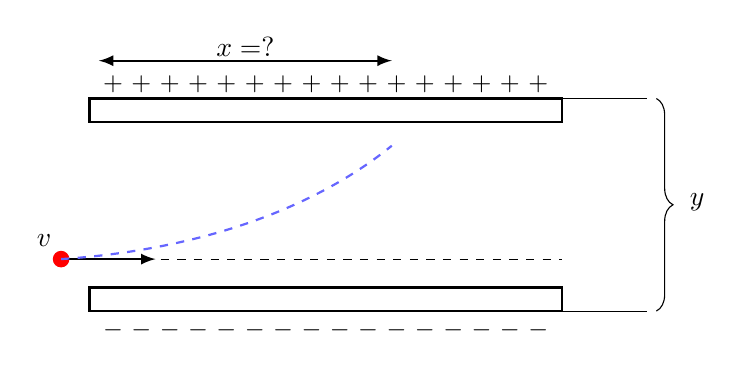
\begin{tikzpicture}[scale=1.2, >=latex]

% Plates
\draw[thick] (0,0) rectangle (5,0.25);
\draw[thick] (0,-2.0) rectangle (5,-1.75);

% Positive charges above upper plate
\foreach \x in {0.25,0.55,...,5.0}
{
    \node at (\x,0.4) {\small $+$};
}

% Negative charges below lower plate
\foreach \x in {0.25,0.55,...,5.0}
{
    \node at (\x,-2.2) {\small $-$};
}

% Electron
\fill[red] (-0.3,-1.45) circle (2.5pt);

% Initial velocity
\draw[->, thick] (-0.25,-1.45) -- (0.7,-1.45);
\node[left] at (-0.3,-1.25) {$v$};

% Dashed horizontal reference line
\draw[dashed] (-0.3,-1.45) -- (5.0,-1.45);

% Curved trajectory
\draw[dashed, thick, blue!60]
    (-0.3,-1.45) .. controls (1.2,-1.35) and (2.4,-0.9) .. (3.2,-0.25);

% x distance arrow
\draw[<->, thick] (0.1,0.65) -- (3.2,0.65);
\node at (1.65,0.8) {$x=?$};

% Vertical bracket for y
\draw[,thin] (5.6,0.25) -- (5.9,0.25);
\draw[thin] (5.6,-2.0) -- (5.9,-2.0);
\draw[decorate, decoration={brace, amplitude=6pt,mirror}]
    (6.0,-2.0) -- (6.0,0.25);
\node[right] at (6.25,-0.85) {$y$};

% Outer light guide lines
\draw[thin] (5.0,0.25) -- (5.6,0.25);
\draw[thin] (5.0,-2.0) -- (5.6,-2.0);

\end{tikzpicture}
%\caption{Electron motion between two parallel charged plates.}
\end{figure}
\end{center}

\pagebreak
The electron enters the electric field with horizontal velocity
$$ v_x = v_0 = 10^6\,\mathrm{m/s}. $$

The vertical acceleration of the electron is
\vskip -10 pt
$$ a_y = \frac{eE}{m_e}. $$

Using
$$ E = 1\,\mathrm{kN/C} = 1000\,\mathrm{N/C}, \qquad m_e = 9.11 \cdot 10^{-31}\,\mathrm{kg}, $$
we obtain
$$ a_y = \frac{1.60 \cdot 10^{-19}\,C \cdot 1000\,N/C} {9.11 \cdot 10^{-31}\,kg} \approx 1.76 \cdot 10^{14}\,\mathrm{m/s^2}. $$

The vertical displacement is
$$ y = \frac{1}{2}a_y t^2, $$

\pagebreak
while the horizontal displacement is
$$ x = v_0 t. $$

Hence,
$$ t = \frac{x}{v_0}. $$

Substituting this into the equation for the vertical motion gives
$$ y = \frac{1}{2}a_y \left(\frac{x}{v_0}\right)^2.$$

Solving for \(x\),
$$ x = v_0 \sqrt{\frac{2y}{a_y}}. $$

\pagebreak
Since
$$ a_y = \frac{eE}{m_e}, $$
the result can also be written as
\vskip -10 pt
$$ \boxed{x = v_0 \sqrt{\frac{2m_e y}{eE}} }.$$

Substituting the numerical constants,
$$ \boxed{ x = 10^6\,m\,\sqrt{\frac{2y}{1.76 \cdot 10^{14}} }}.$$

If \(y\) is measured in metres, then \(x\) is also obtained in metres.

% ----------------------------------------------------------------------------------------------------------------------------------------

\pagebreak
\item An electron enters the region between the plate pair shown in the figure halfway between the plates. The length of the plates is $ l = 8\,\mathrm{cm}, $ their separation is $ d = 1\,\mathrm{cm}, $ and the voltage between them is $ U = 500\,\mathrm{V}. $ What must the initial velocity of the electron be if we want it to just barely leave the region between the plates?

\begin{center}
\begin{figure}[h]
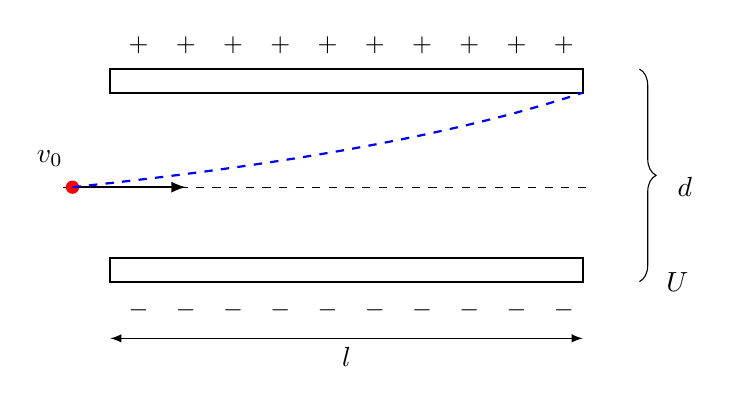
\begin{tikzpicture}[scale=1.2, >=latex]

% Parameters (for clarity)
\def\L{5}    % plate length
\def\d{2}    % plate distance

% Plates
\draw[thick] (0,0) rectangle (\L,0.25);
\draw[thick] (0,-\d) rectangle (\L,-\d+0.25);

% Positive charges (upper plate)
\foreach \x in {0.3,0.8,...,4.8}
{
    \node at (\x,+0.5) {\small $+$};
}

% Negative charges (lower plate)
\foreach \x in {0.3,0.8,...,4.8}
{
    \node at (\x,-2.3) {\small $-$};
}

% Midline (entry level)
\draw[dashed] (-0.5,-\d/2) -- (\L+0.1,-\d/2);

% Electron entry point
\fill[red] (-0.4,-\d/2) circle (2pt);

% Initial velocity
\draw[->, thick] (-0.4,-\d/2) -- (0.8,-\d/2);
\node[left] at (-0.4,-\d/2+0.3) {$v_0$};

% Curved trajectory (just touching upper plate at exit)
\draw[thick, dashed, blue]
    (-0.4,-\d/2) .. controls (1.5,-\d/2+0.2) and (3.5,-0.5) .. (\L,0.0);

% Length l
\draw[<->] (0,-\d-0.6) -- (\L,-\d-0.6);
\node at (\L/2,-\d-0.8) {$l$};

% Distance d (brace)
\draw[decorate, decoration={brace, amplitude=6pt, mirror}]
    (\L+0.6,-\d) -- (\L+0.6,0.25);
\node[right] at (\L+0.9,-\d/2) {$d$};

% Voltage label
\node at (\L+1.0,-\d/2-1.0) {$U$};

\end{tikzpicture}
%\caption{Electron motion between parallel plates (Problem 3).}
\end{figure}
\end{center}
  
\pagebreak  
The electric field between the plates is
$$ E = \frac{U}{d}. $$

Using
$$ U = 500\,\mathrm{V}, \qquad d = 1\,\mathrm{cm} = 0.01\,\mathrm{m}, $$
we get
$$ E = \frac{500\,N/C}{0.01\,m} = 5.0 \cdot 10^4\,{N/C}. $$

The acceleration of the electron is
$$ a = \frac{eE}{m_e} = \frac{eU}{m_e d}. $$

\pagebreak
Therefore,
$$ a = \frac{ 1.60 \cdot 10^{-19}\,C \cdot 500\,N/C} {9.11 \cdot 10^{-31}\,kg \cdot 0.01\,m} \approx 8.78 \cdot 10^{15}\,{m/s^2}. $$

The electron enters halfway between the plates. In order to just leave the region
between the plates, its vertical displacement must be
$$ \frac{d}{2}. $$

Thus,
$$ \frac{d}{2} = \frac{1}{2}at^2. $$

Hence,
$$ d = at^2, \qquad t = \sqrt{\frac{d}{a}}.$$

\pagebreak
The horizontal motion is uniform:
$$ l = v_0 t. $$

Therefore,
$$ v_0 = \frac{l}{t} = l\sqrt{\frac{a}{d}}. $$

Substituting
$$ a = \frac{eU}{m_e d}, $$
we obtain
$$ v_0 = l\sqrt{ \frac{eU}{m_e d^2} }.$$

With
$$ l = 8\,{cm} = 0.08\,{m}, \qquad d = 0.01\,{m}, $$

\pagebreak
this gives
$$ v_0 = 0.08\,m \sqrt{ \frac{ 1.60 \cdot 10^{-19}\,C \cdot 500\,N/C }{9.11 \cdot 10^{-31}\,kg \cdot (0.01\,m)^2 }}\approx 7.50 \cdot 10^6\,{m/s}.$$

Thus,
$$ \boxed{ v_0 \approx 7.5 \cdot 10^6\,{m/s} }.$$

\end{enumerate}


\end{itemize}

\end{frame}

% ----------------------------------------------------------------------------------------------------------------------------------------

\begin{frame}
%\frametitle{Minden jó, ha a vége jó}

\vfill
\begin{center}
\textbf{\huge The End}

\bigskip
Thank you for your attention!
\end{center}
\vfill
%\textbf{Acknowledgements} Thank you for the course materials for Szilárd~ZSÓKA and Zoltán~VARGA.
\end{frame}

\end{document}
